\let\negmedspace\undefined
\let\negthickspace\undefined
\documentclass[journal,12pt,twocolumn]{IEEEtran}
\usepackage{cite}
\usepackage{amsmath,amssymb,amsfonts,amsthm}
\usepackage{algorithmic}
\usepackage{graphicx}
\usepackage{textcomp}
\usepackage{caption}
\usepackage{xcolor}
\usepackage{txfonts}
\usepackage{listings}
\usepackage{enumitem}
\usepackage{mathtools}
\usepackage{gensymb}
\usepackage[breaklinks=true]{hyperref}
\usepackage{tkz-euclide} % loads  TikZ and tkz-base
\usepackage{listings}
\usepackage{gvv}
\newtheorem{theorem}{Theorem}[section]
\newtheorem{problem}{Problem}
\newtheorem{proposition}{Proposition}[section]
\newtheorem{lemma}{Lemma}[section]
\newtheorem{corollary}[theorem]{Corollary}
\newtheorem{example}{Example}[section]
\newtheorem{definition}[problem]{Definition}
%\newtheorem{thm}{Theorem}[section] 
%\newtheorem{defn}[thm]{Definition}
%\newtheorem{algorithm}{Algorithm}[section]
%\newtheorem{cor}{Corollary}
\newcommand{\BEQA}{\begin{eqnarray}}
\newcommand{\EEQA}{\end{eqnarray}}
\newcommand{\define}{\stackrel{\triangle}{=}}
\theoremstyle{remark}
\newtheorem{rem}{Remark}

%\bibliographystyle{ieeetr}
\begin{document}
%

\bibliographystyle{IEEEtran}


\vspace{3cm}

\title{
%	\logo{
Assignment-11.14.7 

\large{EE:1205-Signals and Systems}

Indian Institute of Technology, Hyderabad
%	}
}
\author{Md Ayaan Ashraf

EE23BTECH11041
}	

\maketitle

\newpage

%\tableofcontents

\bigskip

\renewcommand{\thefigure}{\theenumi}
\renewcommand{\thetable}{\theenumi}
%\renewcommand{\theequation}{\theenumi}
\section*{\textbf{\textit{Question}}}
The motion of a particle executing simple harmonic motion is described by the
displacement function, $x(t)$ = $A$ $cos$ ($\omega$$t$ +$\phi$).
If the initial $(t = 0)$ position of the particle is $1 cm$ and its initial velocity is $\omega\quad cm/s$, what are its amplitude and initial phase angle ? The angular frequency of the particle is $\pi\quad s^{-1}$. If instead of the cosine function, we choose the sine function to describe the SHM : $x$ = $B$ $sin$ ($\omega$$t$ +$\alpha$), what are the amplitude and initial phase of the
particle with the above initial conditions.
\section*{\textit{\textbf{Solution}}}

\begin{table}[h]
  \centering
  \begin{tabular}{|c|c|c|}
    \hline
Parameter & Description & Value \\ \hline
$x(0)$ & Initial position of particle & 1cm\\ \hline
$\omega$ & Angular frequency of particle & $\pi s^{-1}$ \\ \hline
$x'(0)$ & Initial velocity of particle & $\omega$ \\ \hline
$\phi$ & Initial Phase Angle & ?\\
\hline
$\alpha$ & New Phase Angle & ?\\
\hline
$A$ & Initial Amplitude & ?\\
\hline
$B$ & New Amplitude & ?\\
\hline
  \end{tabular}
  \vspace{2mm}
  \caption{Parameter Table 11.14.7}
\end{table}



The displacement function for simple harmonic motion (SHM) is given by:
\begin{align}
   x(t) = A \cos(\omega t + \phi)  
\end{align}
Given:
\begin{align}
     x(0)&= A \cos(\phi) = 1 \text{ cm} \\
 x'(0)&= -A \omega \sin(\phi) = \omega \text{ cm/s} \label{eq:3}
 \end{align}
Solving for $\phi$ and $A$:
\begin{align}
    tan(\phi) = -1\\
\implies
\phi = -\frac{\pi}{4} \\
\implies 
A= \sqrt{2}cm
\end{align}
If we choose the sine function instead, the displacement function becomes:
\begin{align}
    x(t) = B \sin(\omega t + \alpha) 
    \end{align}
    Given:\\
    \begin{align}
     B \sin(\alpha) &= 1 \text{ cm} \\
    B \omega \cos(\alpha) &= \omega \text{ cm/s}\label{eq;11}
\end{align}
Solving for $\alpha$ and $B$:
\begin{align}
    tan(\alpha)& = 1\\
\implies
\alpha &= \frac{\pi}{4} \\
\implies 
B &=\sqrt{2}cm
\end{align}
\begin{figure}[h]
\renewcommand\thefigure{1}
    \centering
    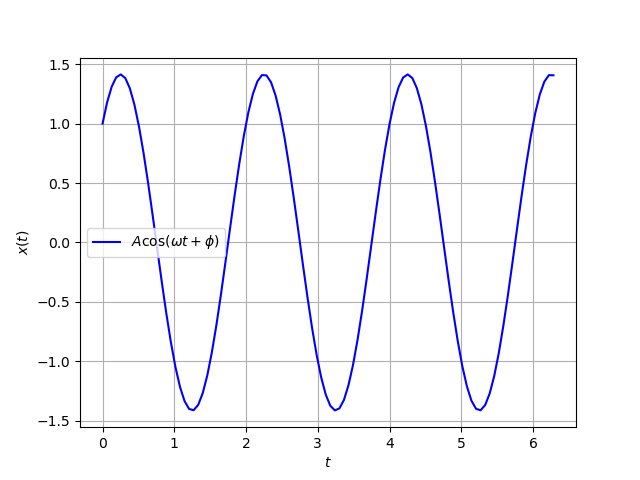
\includegraphics[width=0.8\columnwidth]{figs/fig1.png}
    \caption{$x(t) = \sqrt{2}\cos(\pi t - \frac{\pi}{4}$)}
    \label{Fig1}
\end{figure}
\begin{figure}[h]
\renewcommand\thefigure{2}
    \centering
    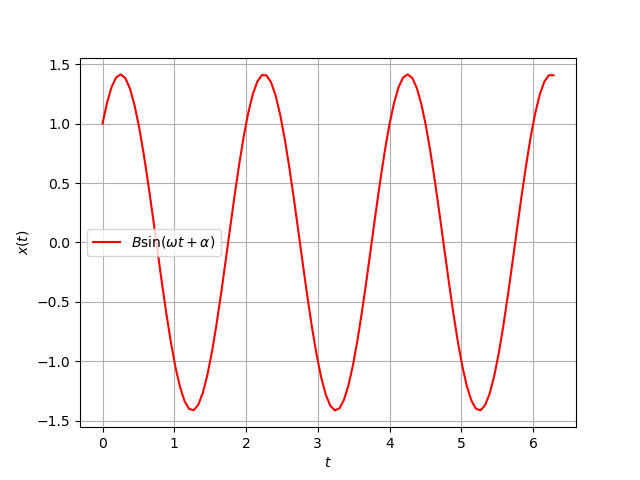
\includegraphics[width=0.8\columnwidth]{figs/fig2.png}
    \caption{$x(t) = \sqrt{2}\sin(\pi t + \frac{\pi}{4})$}
    \label{Fig2}
\end{figure}
\end{document}
